%%%%%%%%%%%%%%%%%%%%%%%%%%%%%%%%%%%%%%%%%%%%%%%%%%%%%%%%%%%%%%%%%%%%%%%%
\documentclass[12pt]{article}
\usepackage{amssymb,amsthm}
\usepackage{amsmath,amssymb,CJK}
\usepackage{graphicx}
\usepackage{subfigure}
\usepackage{listings}
\usepackage{enumerate}

\openup 7pt\pagestyle{plain} \topmargin -40pt \textwidth
14.5cm\textheight 21.5cm
\parskip .09 truein
\baselineskip 4pt\lineskip 4pt \setcounter{page}{1}
\def\a{\alpha}\def\b{\beta}\def\d{\delta}\def\D{\Delta}\def\fs{\footnotesize}
\def\g{\gamma}
\def\G{\Gamma}\def\l{\lambda}\def\L{\Lambda}\def\o{\omiga}\def\p{\psi}
\def\se{\subseteq}\def\seq{\subseteq}\def\Si{\Sigma}\def\si{\sigma}\def\vp{\varphi}\def\es{\varepsilon}
\def\sc{\scriptstyle}\def\ssc{\scriptscriptstyle}\def\dis{\displaystyle}
\def\cl{\centerline}\def\ll{\leftline}\def\rl{\rightline}\def\nl{\newline}
\def\ol{\overline}\def\ul{\underline}\def\wt{\widetilde}\def\wh{\widehat}
\def\rar{\rightarrow}\def\Rar{\Rightarrow}\def\lar{\leftarrow}
\def\Lar{\Leftarrow}\def\Rla{\rightleftarrow}\def\bs{\backslash}
\def\ra{\rangle}\def\la{\langle}\def\hs{\hspace*}\def\rb{\raisebox}
\def\ni{\noindent}\def\hi{\hangindent}\def\ha{\hangafter}
\def\vs{\vspace*}
\def\hom#1{\mbox{\rm Hom($#1,#1$)}}
\def\thebeg{\vskip8pt\par\ni}
\def\theend{\vskip5pt\par}
\def\chabeg{\pagebreak\par}
\def\chaend{\vskip20pt\par}
\def\secbeg{\vskip15pt\par}
\def\secend{\vskip10pt\par}
\def\exebeg{\vskip10pt}
\def\exeend{\vskip6pt}
\def\undot#1{\mbox{$\mbox{#1}\hs{-1.5ex}_{_{\dis\centerdot}}\,\,$}}
\def\qed{\hfill\mbox{$\Box$}}
\def\C{\mathbb{C}}
\def\Q{\mathbb{Q}}
\def\ii{\mbox{\,{\bf i}\,}}
\def\jj{\mbox{\,{\bf j}\,}}
\def\AA{{\cal A}}
\def\BB{{\cal B}}
\def\DD{{\cal D}}
\def\EE{{\mbox{\bf 1}}}
\def\OO{{\mbox{\bf 0}}}
\def\kk{{\mbox{\bf k}}}
\def\R{\mathbb{R}}
\def\F{\mathbb{F}{\ssc\,}}
%\def\similar{\rb{-4pt}{\mbox{\,\~\,}}}
\def\similar{\backsim}
\def\Llra{\Longleftrightarrow}
\def\Lra{\Longrightarrow}
\def\Lla{\Longleftarrow}
\def\mat#1#2{\mbox{$\left(\begin{array}{#1}#2\end{array}\right)$}}
\def\det#1#2{\mbox{$\left|\begin{array}{#1}#2\end{array}\right|$}}
\def\eset{\emptyset}
\parindent=5ex
\setlength{\parindent}{0pt}
\setlength{\parskip}{1ex plus 0.5ex minus 0.2ex}
\newtheorem{Example}{\text{例}}
\begin{CJK*}{UTF8}{gbsn}

\date{}
\title{Homework5}
\author{Qinglin Li, 5110309074}
\begin{document}
\maketitle

\section*{Problem 1}
\begin{enumerate}
\item
Let 
$
Z_v[t]=\left\{
\begin{aligned}
&1~~~\text{vertex }v\text{ changes color at step }t\\
&0~~~\text{otherwise}
\end{aligned}
\right.
$\\
Let $C_t[v]$ be the color of vertex $v$ at step $t$ and $d_v$ be the degree of the vertex $v$\\

Let 
$
\begin{aligned}
W_t&=\left\{v\in V|C_t[v]=\texttt{white}\right\}\\
B_t&=\left\{v\in V|C_t[v]=\texttt{black}\right\}
\end{aligned}
$\\
Let $D_t[v]=\Big|\{u\in V|(u,v)\in E\wedge C_t[u]\neq C_t[v]\}\Big|$, thus
\begin{equation}\label{eq1}
Y_{t+1}-Y_{t}=\sum_{v\in B_t}d_vZ_t[v]-\sum_{v\in W_t}d_vZ_t[v]
\end{equation}
\begin{equation}\label{eq2}
E\left[Z_t[v]\right]=\dfrac{D_t[v]}{2d_v}
\end{equation}
Combine \eqref{eq1} with \eqref{eq2}
$$E\big[Y_{t+1}-Y_t|X_1,\cdots,X_t\big]=\sum_{v\in B_t}d_v\dfrac{D_t[v]}{2d_v}-\sum_{v\in W_t}d_v\dfrac{D_t[v]}{2d_v}=\dfrac{1}{2}\left({\sum_{v\in B_t}D_t[v]-\sum_{v\in W_t}D_t[v]}\right)$$
So
$$E\big[Y_{t+1}-Y_t|X_1,\cdots,X_t\big]=0$$
Then $Y_i$ is a martingale of $\{X_i\}$
\item
$\because |Y_{t+1}-Y_t|\leq 2m$  (the total degree)\\
$\therefore E\left[|Y_{t+1}-Y_t|\big|X_1,\cdots X_{t-1}\right]\leq 2m$\\
Let $T$ be the stopping time, since there exists a system of linear equations of all stopping of all initial states, $E[T]<\infty$\\
By OST, $E[Y_T]=E[Y_0]$\\ 
Let $p$ be the  probability that the process terminates in the all-white configuration\\
$$E[Y_T]=2mp\Rightarrow p=\dfrac{Y_0}{2m}$$
\end{enumerate}

\section*{Problem 2}
\begin{enumerate}
\item
Let $d_v$ be the degree of vertex $v$\\
Define a random walk, $\forall u\in V$\\
$$
\left\{
\begin{aligned}
P(u,v)&=\dfrac{1}{\Delta+1}~~~~~~~~(u,v)\in E\\
P(u,u)&=1-\dfrac{d_u}{\Delta+1}
\end{aligned}
\right.
$$

Since $P(u,u)>0$, the random walk is a aperiodic, then ergodic.\\

For uniform distribution $\pi$, $\forall u,v\in V \wedge (u,v)\in E, \pi_uP(u, v)=\pi_vP(v, u)$, So the random walk is time reversible.\\

$\forall (u,v)\in E, P(u,v)>0 \Rightarrow$ the random walk is irreducible\\
By fundamental theorem of markov chain\\
 irreducible $+$ ergodic $\Rightarrow$ stationary distribution is unique $\Rightarrow$ stationary distribution is the uniform distribution
\item
$\forall u\in V$, let $S_u=\sum_{(u,v)\in E}\pi_v$\\
$$
\left\{
\begin{aligned}
P(u,v)&=\dfrac{\pi_v}{2}~~~~~~~~(u,v)\in E\\
P(u,u)&=1-\dfrac{S_u}{2}
\end{aligned}
\right.
$$
By similar process, it can be proved that 
\end{enumerate}

\section*{Problem 3}
The original process is equal to choosing a number $i$ uniformly at random from $\{1,2,\cdots,n+1\}$ and then changing $b_i$ if $i\neq n+1$\\
For two process $X_t, Y_t$, at each step, define the following coupling\\
\begin{enumerate}
\item
If $i\neq n+1\wedge X_t[i]=Y_t[i]$, flip $X_t[i]$ and $Y_t[i]$
\item
If $i=n+1 \vee X_t[i]\neq Y_t[i]$, let $I=\{i|X_t[i]\neq Y_t[i]\}\cup\{n+1\}=\{i_1,i_2,\cdots,i_{m}=n+1\}$\\
Define $f:I\rightarrow I$
$$f(i_x)=i_{(x\mod m)+1}$$
Then flip $X_t[i]$ and $Y_t[f(i)]$\\
\end{enumerate}
Every time (2) happens, then hamming distance of $X_t$ and $Y_t$ decreases by at least 1\\
So this coupling is equal to an coupon collector model\\
The mixing time should be $O(n\ln n)$

\section*{Problem 4}
\begin{enumerate}
\item
\textbf{Irreducible}\\

It is supposed to prove that it is reachable from any coloring $C$ to any coloring $D$\\
Induction on $n$\\

If $n=1$, then $\D=0$ irreducible is satisfied by two colors\\
If $n>1$, suppose $\forall G\text{ with }n'<n, \D'<\D$ is irreducible
\begin{enumerate}
\item
If there exists an vertex $v$ with color $\D+2$, choose arbitary $c\in\{1,2,\cdots\D+1\}\setminus\{\text{color of $v$'s neighbor}\}$ and change the color of $v$ to c\\
($c$ always exists since the maximum degree of $v$ is $\D$)\\

Repeat this process until there exists no vertex with color $\D+2$ and the whole process can be finished in finite steps\\
Apply the whole process on $C$ and $D$, then get $C'$ and $D'$\\
Since the process is reversible, the reachability of $C$ and $D$ cannot change\\
\item
Let $V_\D\subset V$ be all verteces with degree $\D$\\
If $V_\D\neq \emptyset$, let $T$ be a maximum independent set on $V_\D$, then $G-T$ has no vertex with degree of $\D$\\
(Otherwise some vertex with degree $\D$ in $G-T$ has no neighbor with degree $\D$ in $G$ implying that $T$ is not a maximum indepentdent set)
If $V_\D=\emptyset$ let $T$ be any nonempty independent set of $G$\\
\item
Since $G-T$ has $n'<n, \D'<D$, it is reachable from $C'$ to $D'$\\
\item
change the color on $T$
\end{enumerate}
Thus it is reachable from $C$ to $D$\\

\textbf{Aperiodic}\\

For any state, because it is non-zero probability doing nothing, aperiodic holds\\

\textbf{Time reversible}\\

$\forall x,y\in \Omega, P(x,y)>0$ iff at most one vertex has different color\\
If $x=y$, $P(x,y)=P(y,x)$\\
If one vertex has different color, since the probability of choosing that vertex is equal in both states, $P(x,y)=P(y,x)$\\
$\therefore \forall x,y\in \Omega, \pi_xP(x,y)=\pi_yP(y,x)$\\
$\therefore$Time reversible\\

\textbf{The stationary distribution is the uniform distribution}\\

$\because \pi$ in time reversible proof is stationary distribution\\
$\therefore$ By fundamental teorem of markov chain the stationary distribution is unique \\
$\therefore$ The stationary distribution is the uniform distribution
\item
Consider $\D=2, q=3$

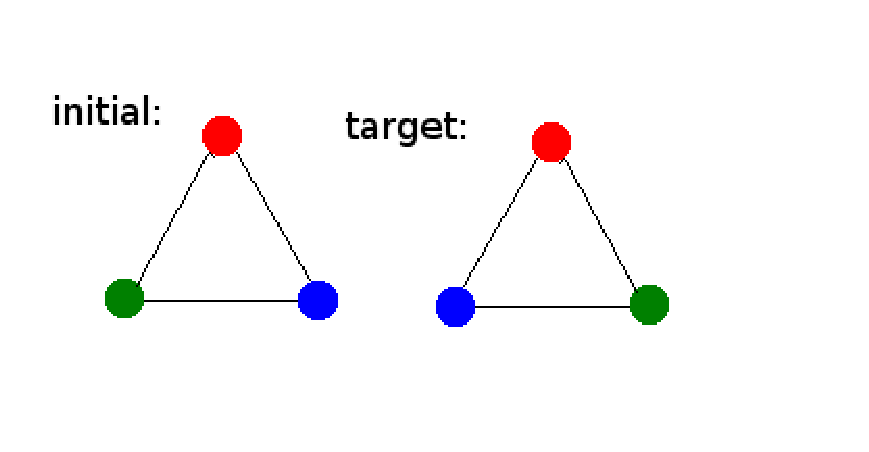
\includegraphics[scale=0.8]{a}\\

\end{enumerate}
\section*{Problem 5}
\begin{enumerate}
\item
\textbf{Ergodic}\\

$\forall 0<p<1,$ because the probability of doing nothing is nonzero, it is aperiodic then is ergodic\\

\textbf{Time reversible}\\

$\forall x,y \in \Omega, P(x,y)>0$ iff at most one element of $x$ and $y$ is different\\
If $x=y$, $P(x,y)=P(y,x)$\\
If one element of $x$ and $y$ is different, since the probability of choosing that element is equal in both $x$ and $y$, $P(x,y)=P(y,x)$\\
Therefore, $\forall x,y\in \Omega, \pi_xP(x,y)=\pi_yP(y,x)$. So it is time reversible\\

\textbf{The stationary distribution is the uniform distribution}\\

$\because \pi$ in time reversible proof is stationary distribution\\
$\therefore$ By fundamental teorem of markov chain the stationary distribution is unique \\
$\therefore$ The stationary distribution is the uniform distribution\\
\item
For two markov chains $X_t$ and $Y_t$, define the following coupling\\
At step $t$, $X_t$ do nothing with probability $p$\\
\begin{enumerate}
\item
If $X_t$ do nothing, $Y_t$ do nothing as well\\
\item
Otherwise choose $a',b'$ for $Y_t$ as follow\\
\begin{enumerate}
\item
If $a\in Y_t$, $a'=a$ else randomly choose $a'$ in $Y_t\setminus X_t$
\item
If $b\in [n]-S_2$, $b'=b$ else randomly choose $b'$ in $\overline{Y_t}\cap X_t$
\end{enumerate}
$X_{t+1}=X_t-{a}+{b}$\\
$Y_{t+1}=Y_t-{a'}+{b'}$\\
Let $D_t=\Big|X_t\setminus Y_t\Big|$\\
At each step, if $a'\neq a$ or $b'\neq b$, $D_t$ decreases by at least $1$\\
\begin{align*}
&\Pr(D_t \text{ decreases by at least } 1)\\
=&(1-p)\left(1-\Pr(a\in X_t\cup Y_t)\Pr(b\in \overline{X_t}\cup\overline{Y_t})\right)\\
=&(1-p)\left(1-\dfrac{k-D_t}{k}\cdot\dfrac{n-k-D_t}{n-k}\right)\\
\leq&(1-p)\dfrac{D_t}{k}
\end{align*}
Thus the upperbound of mixing time is 
$$\sum_{i=1}^k \dfrac{k}{1-p}\dfrac{1}{i}=\dfrac{1}{p}k\ln k=O(n\ln k)$$
So mixing time is asymptotically $O(n\ln k)$ or less
\end{enumerate}
\end{enumerate}
\end{CJK*}
\end{document}